\chapter{Introduction}\label{chap:introduction}
In times where computational tasks are becoming increasingly heavy, many systems require multiple servers or computers to complete these tasks. These servers, or computers, often referred to as nodes, interact directly with each other, are decentralized, and form a so-called Peer-to-Peer network. As depicted in figure \ref{fig:setting}, each node consists of a CPU, a memory module, and a network interface for communication with other nodes. Together, these nodes form a scalable network. The memory system is modeled as a distributed memory scheme, where each node has its own memory module, rather than a shared one, in order to avoid bottlenecks in memory access. \cite{ChengzhongFrancis}

Each computer is assigned a non-negative workload, referred to as load, which can represent various computational tasks such as CPU usage, memory utilization, or internet traffic \cite{Dinitz2023DAB}. The main objective when applying load balancing algorithms is to balance the state of the network, meaning that each node holds the average load of the network. This is accomplished by addressing overloading and underloading through the redistribution of load to other nodes. Heavily overloaded nodes risk failing to complete their tasks due to overheating. Therefore, load balancing enhances coordination in distributed systems and improves scalability.

\begin{figure}[]
    \centering
    \scalebox{0.3}{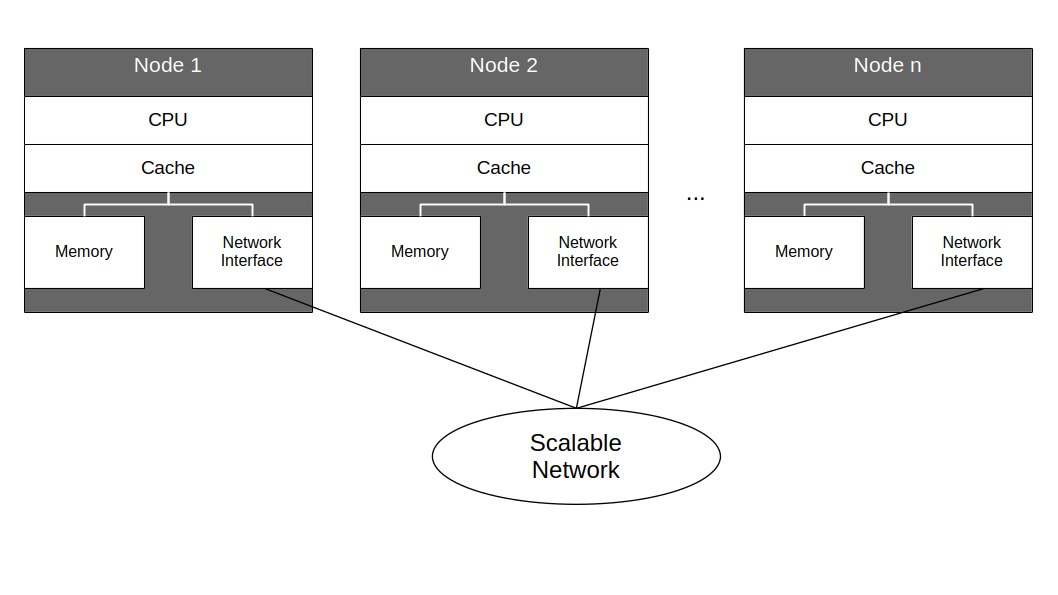
\includegraphics{figures/Diagrams/Setting.png}}
    \caption{Overview of the setting}
    \label{fig:setting}
\end{figure}

\section{Preliminaries}\label{sec:prelimn}
The following definitions are taken from the lecture slides of Graph Theory of the summer term 2021 \cite{GraphTheorySchindelhaauer2021}:
\begin{definition}[General Graph]
    A graph $G$ is defined as $G = (V, E \subseteq V \times V)$, where $V := \{v_0, v_1,...\}$ represents the \textit{vertices} (or nodes) of $G$ and $E := \{e_0, e_1,...\}$ represents the \textit{edges}. The graph may consist of a single vertex and no edges.
\end{definition}

\begin{definition}[Order, Incident, Degree]
    The number of vertices $|V|$ in the graph is referred to as the \textit{order} of $G$.
    
    A vertex and an edge are \textit{incident} if the vertex is an endpoint of the edge.
    
    The \textit{degree} of a vertex is the number of incident edges.
\end{definition}

\begin{definition}[Regular Graphs]
    A \textit{regular graph} is a graph where each vertex has the same degree.
\end{definition}

\begin{definition}[Adjacent]
    If an edge connects two vertices, these vertices are \textit{adjacent} to each other, thus are neighboring vertices.
\end{definition}

\begin{definition}[Loop, Multiple Edges, Simple Graph]
    A \textit{loop} is an edge that connects a vertex to itself.
    
    \textit{Multiple edges} refer to edges that share the same pair of endpoints.
    
    The \textit{simple graph} is a graph that has no loops or multiple edges.
\end{definition}

\begin{definition}[Clique]
    A \textit{clique} is a set of pairwise adjacent vertices. So a subgraph of $G$ that is complete.
\end{definition}

\begin{definition}[Path]
    A \textit{path} is a simple graph whose vertices can be ordered such that two vertices are adjacent if and only if they are consecutive in the list.
\end{definition}

\begin{definition}[Connected Graphs]
    \textit{Connected graphs} are graphs where each pair of vertices in the graph belongs to a path.
\end{definition}

\begin{definition}[Bipartite Graphs]
    \textit{Bipartite graphs} are graphs where the set of graph edges is the union of two disjoint independent sets.
\end{definition}

\begin{definition}[Distance, Diameter]
    If $G$ has a path from node $u$ to node $v$, then the \textit{distance} from $u$ to $v$, $d_G(u,v)$, is the shortest length from a $u,v$-path.
    
    The \textit{diameter} of the graph $\text{diam} (G) := max_{u,v\in V}d_G(u,v)$ is the greatest length of any of the shortest paths between any two nodes.
\end{definition}

\begin{definition}[Peer-to-Peer Network]
    A \textit{Peer-to-Peer Network (P2P)} is a communication network between computers on the internet without a central control and without reliable partners \cite{Peer2PeerSchindelhaauer2023}.
\end{definition}

\section{Motivation}\label{sec:motivation}
The motivation for this thesis stems from the observed performance discrepancies between the Single-Proposal Deal-Agreement-Based algorithm proposed by Yefim Dinitz, Shlomi Dolev, and Manish Kumar \cite{Dinitz2023DAB} and the Push-Pull Sum algorithm described in the paper by Saptadi Nugroho, Alexander Weinmann, and Christian Schindelhauer \cite{nugroho2023PushPullSumDataAg} across different network topologies. These observations were initially gathered during the student project titled "Comparative Analysis of Load Balancing Algorithms in General Graphs" \cite{Bayazitoglu}. According to the simulations conducted in the student project, the Push-Pull Sum algorithm performs better in reducing the MSE per round for the Complete graph and the Star graph compared to the Deal-Agreement-Based algorithm, which performs better in reducing the MSE per round for the Torus Grid graph and the Ring graph. The simulations were conducted for different network sizes, which also influenced the convergence speed, with larger network sizes requiring more rounds to achieve balance.

To address these challenges, this thesis introduces the Adaptive Threshold Push-Pull Sum algorithm, which combines the strengths of both the Continuous Single-Proposal Deal-Agreement-Based and the Push-Pull Sum algorithms and establishes a trade-off to lessen their respective drawbacks. The introduced algorithm uses the mechanic of adaptive thresholding in order to prevent load transfers with low effect in error reduction, since load transfers are pricey operations. This approach bridges the gap between the two algorithms by adjusting to the network's current state of balance.

\section{Related Work}\label{sec:relatedwork}
Nugroho et al. \cite{nugroho2023PushPullSumDataAg} proposed the Push-Pull Sum algorithm, which is essentially a combination of two algorithms: the Push-Sum algorithm, introduced by David Kempe, Alin Dobra, and Johannes Gehrke \cite{kempe2003gossipbasedComp}, and the Pull-Sum algorithm. The push and the pull mechanisms are directly adopted from the Push-Pull Sum algorithm. Nugroho et al. use the MSE as a metric to evaluate the performance of their algorithm, an approach that will also be followed in this thesis. Their experiments were conducted on static general graphs, and this thesis similarly analyzes the behavior of the load balancing algorithms in static graphs.

Dinitz et al. \cite{Dinitz2023DAB} proposed two versions of the Single-Proposal Deal-Agreement-Based algorithm, as well as two variations of a multi-neighbor load balancing algorithm: a round-robin approach and a self-stabilizing load balancing algorithm. However, the only algorithms comparable to ours are the Single-Proposal Deal-Agreement-Based algorithms, which have two variations: one for the continuous setting and one for the discrete setting. The main difference between these two is that, in the continuous setting, any load may be transferred over the edges, whereas, in the discrete setting, all load transfers must involve integers. For multi-neighbor load balancing, nodes may transfer loads to several neighbors within a single round. In contrast, the Push-Pull Sum algorithm allows this only during pull actions, where a node responds to all requesting nodes by sending loads back. Additionally, the self-stabilizing and round-robin approaches are asynchronous algorithms, whereas both the Adaptive Threshold Push-Pull Sum and the Push-Pull Sum algorithms operate synchronously.

\section{Hypothesis}\label{sec:hypothesis}
The Adaptive Threshold Push-Pull Sum algorithm, which integrates key features of the Deal-Agreement-Based algorithm and the Push-Pull Sum algorithm, will demonstrate performances that are intermediate between the two in terms of MSE reduction across six network topologies. Specifically, it is expected to perform better than the Deal-Agreement-Based algorithm in reducing the error in high-degree networks and perform better than the Push-Pull Sum algorithm in reducing the error in low-degree networks.

This hypothesis will be evaluated through a comparative analysis of MSE across six topologies, some of which feature varying network sizes, to evaluate the algorithm's scalability. To analyze the data trends and draw conclusions about the convergence rate, model fitting is applied as an analysis technique. Additionally, slopes will be computed for three distinct time regions—\textit{start}, \textit{middle}, and \textit{end}—to provide insights into the algorithm's performance at specific stages of execution.

\section{Contribution}\label{sec:contribution}
This thesis introduces a novel load balancing algorithm that combines the strengths of two established approaches: randomized load balancing and load balancing based on deal agreement. The introduced algorithm uses an adaptive threshold mechanism in order to adjust to the current state of the network to enhance performance. The push and pull mechanisms are directly adopted by the Push-Pull Sum algorithm.